\subsection{Introdução ao conceito \textit{Zero Energy}}
Define-se que um edifício \textit{Zero Energy} – ZEB, ou em português, balanço 
energético nulo, é uma edificação  energeticamente  eficiente  onde,  
considerada  a  fonte  energética,  a  energia  elétrica fornecida pela 
concessionária é anualmente menor ou igual à quantidade de energia renovável 
exportada pela edificação para a rede 
\cite{Torcellini2006,U.S.DepartmentofEnergy-USDOE2012,U.S.DepartmentofEnergy-USDOE2015}.\vspace*{0.3cm} \newline
\textcite{Domingos2014} define  que  o  balanço  energético  nulo  pressupõe  
uma  arquitetura adequada ao uso de elementos construtivos e equipamentos 
de alta eficiência energética, aliado ao desempenho da fonte geradora de 
energia elétrica a partir de fontes renováveis.\newline A redução do consumo de 
energia em novas edificações ou em processo de melhoria pode ser alcançada 
por meio de projetos integrados à tecnologias de produção de energia, com 
adoção de soluções   energeticamente   eficientes,   e   por   programas   
de   economia   de   energia \cite{U.S.DepartmentofEnergy-USDOE2015}.\vspace*{0.3cm} \newline
\textcite{Torcellini2006} estabelecem quatro definições acerca das formas de 
se atingir o ZEB em edificações  de  baixo  consumo  de  energia,  ou  
comumente  denominadas \textit{Low-Energy Buildings}. Dentre as formas estudadas estão: 
    \begin{itemize}
        \item \textit{Zero Site Energy}, ou energia local zero ou ainda energia da 
        edificação \cite{U.S.DepartmentofEnergy-USDOE2015}, onde é avaliada a 
        potencialidade de produção de energia elétrica para a  edificação  
        utilizando  os  recursos  presentes  no  local,  ou on-site,  onde  o  
        edifício  está implantado. É minimamente avaliado o consumo dos 
        sistemas de condicionamento de ar, de aquecimento quando existente, 
        ventilação, cargas de equipamentos e de sistema de iluminação;
        \item \textit{Zero Source Energy},  ou  fonte  de  energia  zero,  trata-se  do  
        conceito  onde  é  levado  em consideração toda a cadeia de produção 
        total anual de energia utilizada pela edificação e de consumo de 
        energia primária do edifício. Esta avaliação leva em conta a 
        eletricidade, combustíveis utilizados em processamento e transporte de 
        materiais e componentes para o local da edificação, entre outros aspectos;
        \item \textit{Zero Energy Cost}, ou custo de energia zero, é avaliada a razão, 
        no mínimo igual, entre a quantidade total de dinheiro que é arrecadado 
        com a venda de energia produzida on-siteà  concessionaria,  e  a  
        quantidade  total  paga  pela  utilização  de  serviços  e  energia 
        consumida ao longo do ano; e 
        \item \textit{Zero Energy Emissions},  ou  emissão  zero,  onde  a  edificação  
        produz  uma  quantidade  de energia  renovável  livre  de  emissão  
        de  GEE  ao  menos  igual  a  quantidade  de  energia consumida 
        proveniente de fontes de energia emissoras de GEE. 
    \end{itemize}
As definições descritas para o ZEB, que avaliam fontes de energia variadas, 
os custos atrelados à implantação da edificação, a avaliação do ciclo de vida 
dos materiais e componentes, assim como emissões de GEE, demandam pesquisas e 
desenvolvimento de metodologia particular para cada meio de avaliação. 
Portanto, para este trabalho foi estabelecido o recorte de avaliação para 
as edificações utilizando recursos on-site, classificado como \textit{Zero Site Energy}. 
Tal recorte justifica-se em função da exclusividade dada pela definição 
sobre a utilização de fontes de energia renováveis locais, 
disponíveis no sítio onde a edificação foi implantada, utilizada para pesquisa 
em detrimento das outras definições que tratam de formas de avaliação não 
abordadas nesta pesquisa.\vspace*{0.3cm} \newline
\textcite{Didone2014} e \textcite{Athienitis2015} definem que o planejamento de 
uma edificação \textit{Zero Energy} considera a integração de estratégias energéticas 
e soluções passivas; de otimização da edificação em seu projeto, execução e 
operação; e a utilização de tecnologia de produção de energia solar 
fotovoltaica, entre outras formas de produção de energia, considerando a 
forma da edificação e soluções que aproveitem a disponibilidade de energia 
elétrica solar para o meio urbano, aquecimento solar e luz natural.\vspace*{0.3cm} \newline
A \textcite{InternationalEnergyAgency-IEA2014} publicou um estudo detalhado de 
30 edificações \textit{Zero Energy} em vários países e em diversas situações climáticas. 
O \textit{“Towards Net Zero Energy Solar Buildings: A review of 30 Net ZEBs case studies”} 
foi parâmetro para o desenvolvimento de referências para o planejamento de edificações 
energeticamente nulas. Este estudo concluiu que é possível atingir o balanço energético 
nulo para diversos usos residenciais e comerciais da realidade construtiva americana.\vspace*{0.3cm} \newline
A respeito da nomenclatura utilizada para descrever uma edificação que atinge 
o equilíbrio entre consumo e produção de energia, na série de Guias Avançados de Projeto 
Energético – AEDG \cite{AmericanSocietyofHeatingRefrigeratingandAir-ConditioningEngineers-ASHRAE2019} 
há a utilização do termo \textit{Zero Energy} em oposição aos termos \textit{Net Zero Energy} 
e \textit{Zero Net Energy} em consonância com os termos utilizados pelo Departamento 
de Energia dos Estados Unidos, da mesma forma para as políticas federais e municipais 
de desempenho energético em vigor. O Departamento de Energia dos Estados Unidos também 
utiliza o termo \textit{Zero Energy} justificando que a inserção de “\textit{Net}” não 
adiciona significado substancial a expressão \cite{U.S.DepartmentofEnergy-USDOE2015a}. 
Este trabalho utilizou a nomenclatura em consonância com a AEDG da norma americana ASHRAE 
e demais artigos científicos que adotam \textit{Zero Energy} como balanço energético nulo.

\subsubsection{\textit{Near Zero Energy}}
 Baseado na norma europeia EN 15603:2008, a definição sobre o conceito proposta por
 \textcite{Kurnitski2011a} para edificações \textit{Near Net Zero Energy}, nZEB, e 
 em português, próximo ao balanço energético nulo, se apoia na premissa do aproveitamento 
 máximo de recursos para produção de energia, implementando mecanismos à edificação 
 de forma que este aproveitamento aconteça, e a utilização à nível ótimo da energia 
 primária, para um consumo maior que 0 kWh/m² ao ano. Segundo os autores, são pontos 
 importantes para atender a definição do conceito:
    \begin{itemize}
        \item O custo otimizado e considerável aproveitamento técnico do uso da energia primária; e
        \item A porcentagem de energia primária coberta pela geração de energia proveniente de 
        fontes renováveis.
    \end{itemize}
A nomenclatura adotada, tal qual para \textit{Zero Energy}, foi \textit{Near Zero Energy}, 
em concordância com a nomenclatura encontrada nos estudos consultados e com o termo 
\textit{Zero Energy} adotado anteriormente \cite{AmericanSocietyofHeatingRefrigeratingandAir-ConditioningEngineers-ASHRAE2019}.
Esta variação do conceito de balanço energético nulo é adotada como parâmetro de avaliação 
para a presente pesquisa, uma vez que se adequa ao cenário energético e tecnológico do 
recorte territorial estabelecido, ou seja, a Região Metropolitana da Grande Vitória, no 
Espírito Santo.

\subsubsection{Métrica para balanço energético nulo}
Um edifício energeticamente balanceado produz, consome e, eventualmente, exporta energia
para a concessionária quando as condições climáticas e energéticas são favoráveis para 
este cenário. A avaliação depende de definição do espaço utilizado para geração de energia, 
\textit{on-site} ou \textit{off-site}, e do tempo avaliado deste processo, horário, 
mensal ou, mais comumente, anual \cite{AmericanSocietyofHeatingRefrigeratingandAir-ConditioningEngineers-ASHRAE2019}.\vspace{0.5cm} \newline
Métodos de avaliação foram desenvolvidas para contemplar as variações de se atingir o 
balanço energético nulo como demanda/geração de energia e exportação/importação de energia. 
O primeiro método é direcionado ao \textit{Zero Site Energy}, o que permite avaliar 
anualmente as opções de produção de energia elétrica \textit{on-site} e a demanda de 
energia calculada. O segundo método é normalmente aplicado ao \textit{Zero Source Energy}, 
onde são balanceadas as fontes de energia, carga de energia e interação com a rede da 
concessionária \cite{Didone2014a}.\vspace{0.3cm} \newline
Para tal, é determinada a interação energética entre a concessionária e a edificação, 
como observado na Figura \ref{fig:figura1}.\newline
    \begin{figure}[ht]
    \centering
    \caption{\small Diagrama de interação entre a edificação e as variáveis externas.}
    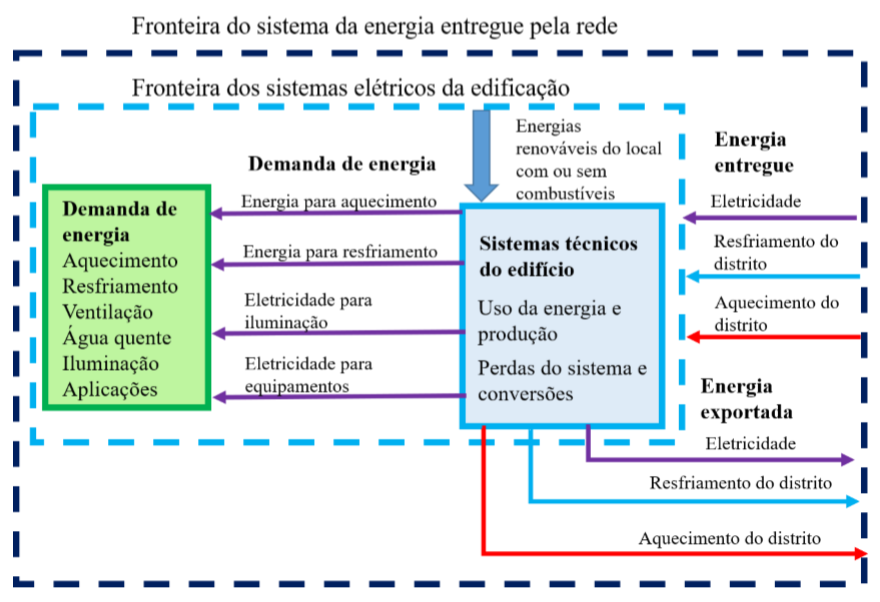
\includegraphics[width=0.85\textwidth]{figures/esquema_kurnitski _2011.png}
    \begin{flushleft}
        \par Fonte: adaptado de Kurnitski et al. (2011, tradução nossa)\small 
    \end{flushleft}\vspace{-0.5cm}
    \label{fig:figura1}
    \end{figure}

\noindent Foram desconsideradas as medidas que envolviam sistema de aquecimento, por não condizer 
com a realidade observada no recorte territorial e por ser uma medida de inclusão facultativa 
em regulamentações nacionais \cite{InstitutoNacionaldeMetrologiaNormalizacaoeQualidadeIndustrial-INMETRO2018,InstitutoNacionaldeMetrologiaNormalizacaoeQualidadeIndustrial-INMETRO2018a}.
De forma a estabelecer a métrica necessária para a avaliação do balanço energético da edificação, 
devem ser conhecidos os componentes de uso final de energia, a energia primária total utilizada 
pela edificação, os custos com o consumo de energia elétrica, e a quantidade de energia 
exportada à concessionária. Da mesma forma, devem ser definidos o período de balanço a ser 
analisado e eventuais créditos provenientes de fornecimento de energia à concessionária. 
Esta relação é ilustrada no Gráfico 1.%\vspace*{-0.1cm}

    \begin{graph}
        \par \small Gráfico 1 - Relação entre demanda energética e créditos para edificação NZEB.
        \begin{minipage}[ht]{1\textwidth}\centering
            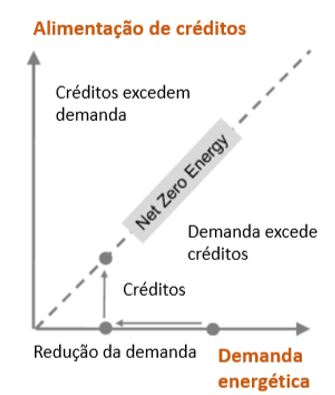
\includegraphics[width=0.3\textwidth]{figures/esquema_iea_2014-2.png}            
        \end{minipage}
        \begin{flushleft}
            \par \small Fonte: adaptado de Kurnitski et al. (2011, tradução nossa).            
        \end{flushleft}
    \end{graph}